\section{Evaluation}
\label{sec:eval}
To assess the effectiveness of TinyNet, we employ our hardware testbed, focusing on accurately timing key message passing intervals and associated delays. These empirical measurements serve to calibrate and inform our simulation model. The simulation, in turn, facilitates rapid iteration across a variety of network traffic scenarios. It enables us to meticulously analyze and quantify the routing paths of messages within the network, offering a detailed insight into TinyNet's performance under different conditions. This combined approach of practical testing and simulation provides a comprehensive evaluation of TinyNet's capabilities.

\subsection{Hardware}
For our hardware evaluation, we utilized the Saleae Logic 8 Logic Analyzer to capture logic level voltages from the microcontrollers. This was crucial for monitoring the router firmware at both the application and networking layers, where pin states (high or low) are indicative of significant event occurrences.

\subsubsection{Processing Delay}
\begin{figure*}[th]
    \centering
    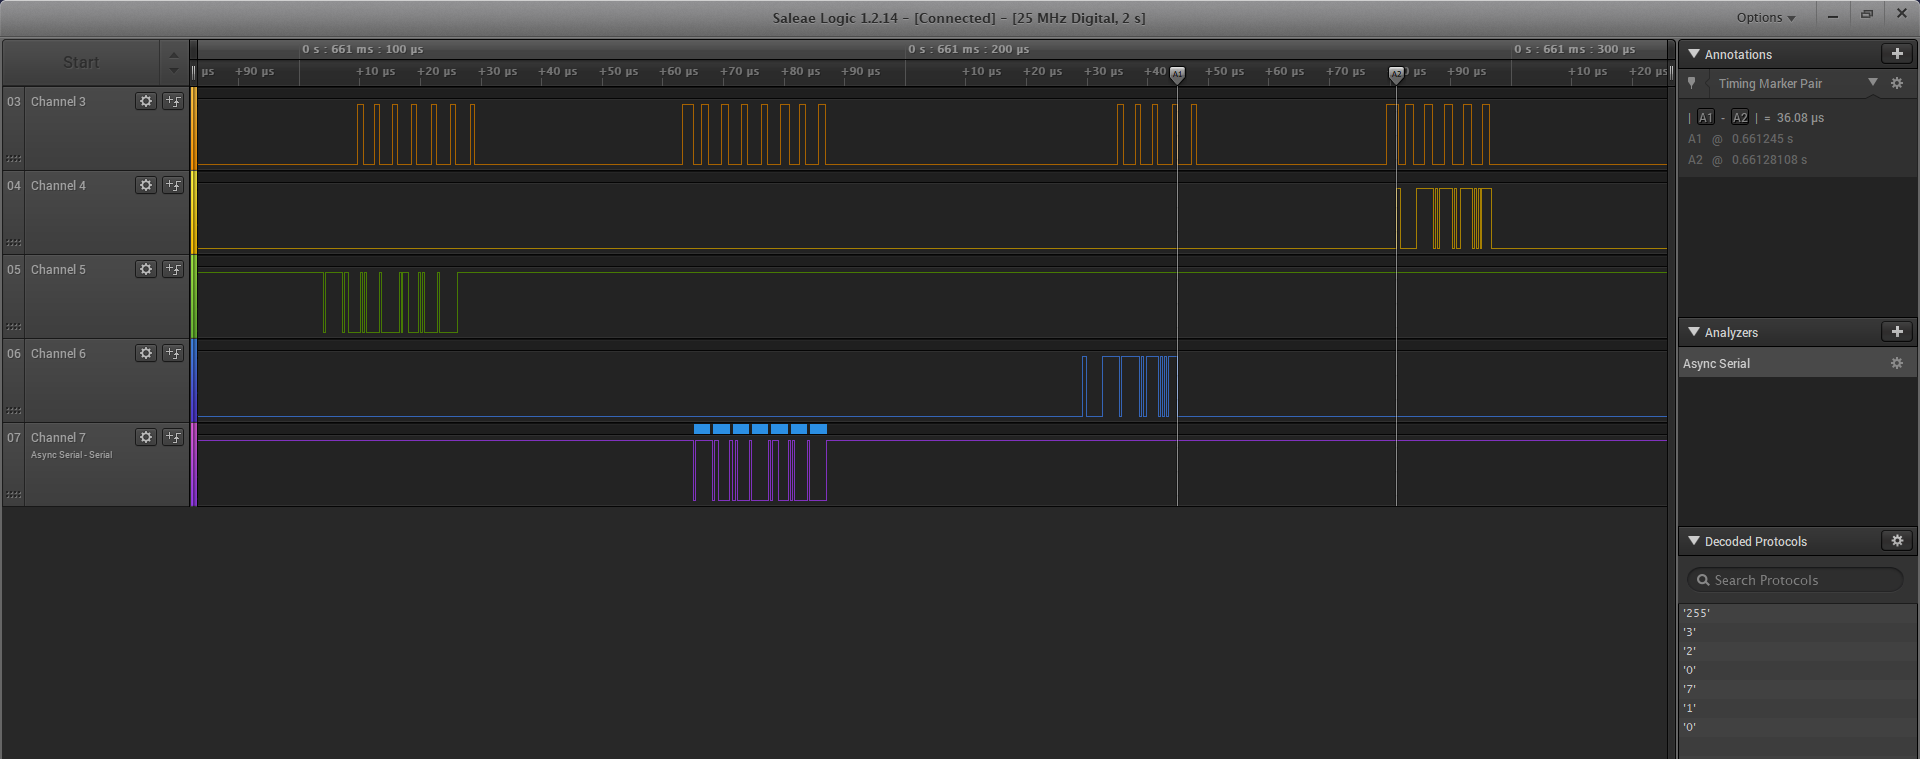
\includegraphics[width=\textwidth]{figures/results-D_p.png}
    \caption{Logic-analyzer capture showing $\mathrm{D}_{\mathrm{process}}$ measurement. Channels show UART activity: Channel 1 = incoming packet end, Channel 2 = outgoing packet start; the interval between them is $\mathrm{D}_{\mathrm{process}} = 37\,\mu\mathrm{s}$. Channel 3 shows per-byte interrupt handling ($\mathrm{D}_{\mathrm{byte}} = 1.5\,\mu\mathrm{s}$).}
    \label{fig:packet-delay}
\end{figure*}
Processing Delay, denoted $\mathrm{D}_{\mathrm{process}}$, is defined as the duration required for a router to determine the appropriate port for forwarding a received packet. To characterize this delay, we recorded signals at the link layer using the logic analyzer, tracking a packet's journey through a single router. Specifically, $\mathrm{D}_{\mathrm{process}}$ was measured as the interval between the end of an incoming packet and the start of the outgoing packet's transmission. By averaging results from 10 such packet traversals, we determined an average processing delay of $37 \mu\mathrm{s}$. The small sample size is justified by the deterministic nature of the MCU's execution path: the forwarding logic executes the same instruction sequence for every packet and runs at the exclusive priority of the main loop, with no competing interrupts during processing. Accordingly, trial-to-trial variation is negligible and the 10-sample mean is representative.

\subsubsection{Link Transmission Time}
Link Transmission Time, defined in equation~(\ref{eq:ltt}) as $\mathrm{L}_{\mathrm{tt}}$, is the time taken for a packet to travel across a link. This calculation was verified using a logic analyzer. The transmission and reception of bytes also consume processor time. As the UART link handles bit-shifting asynchronously on each port, each received character triggers an interrupt requiring processor attention. We measured this interrupt handling time to be $\mathrm{D}_{\mathrm{byte}}=1.5 \mu \mathrm{s}$ per byte, consistent across all tested packets. This value can also be derived analytically: at 300 MHz with the interrupt service routine requiring approximately 450 clock cycles for context save, buffer copy, and return, the expected handling time is $450/300\,\mathrm{MHz} = 1.5\,\mu\mathrm{s}$, confirming the measured result. This process is depicted in Fig.~\ref{fig:packet-delay}, Channel 3. We discuss in Section~\ref{sec:sim-val} how we account for these delays to align our simulation results with our hardware findings.

\subsubsection{Router Behavior}
\begin{figure}[th]
    \centering
    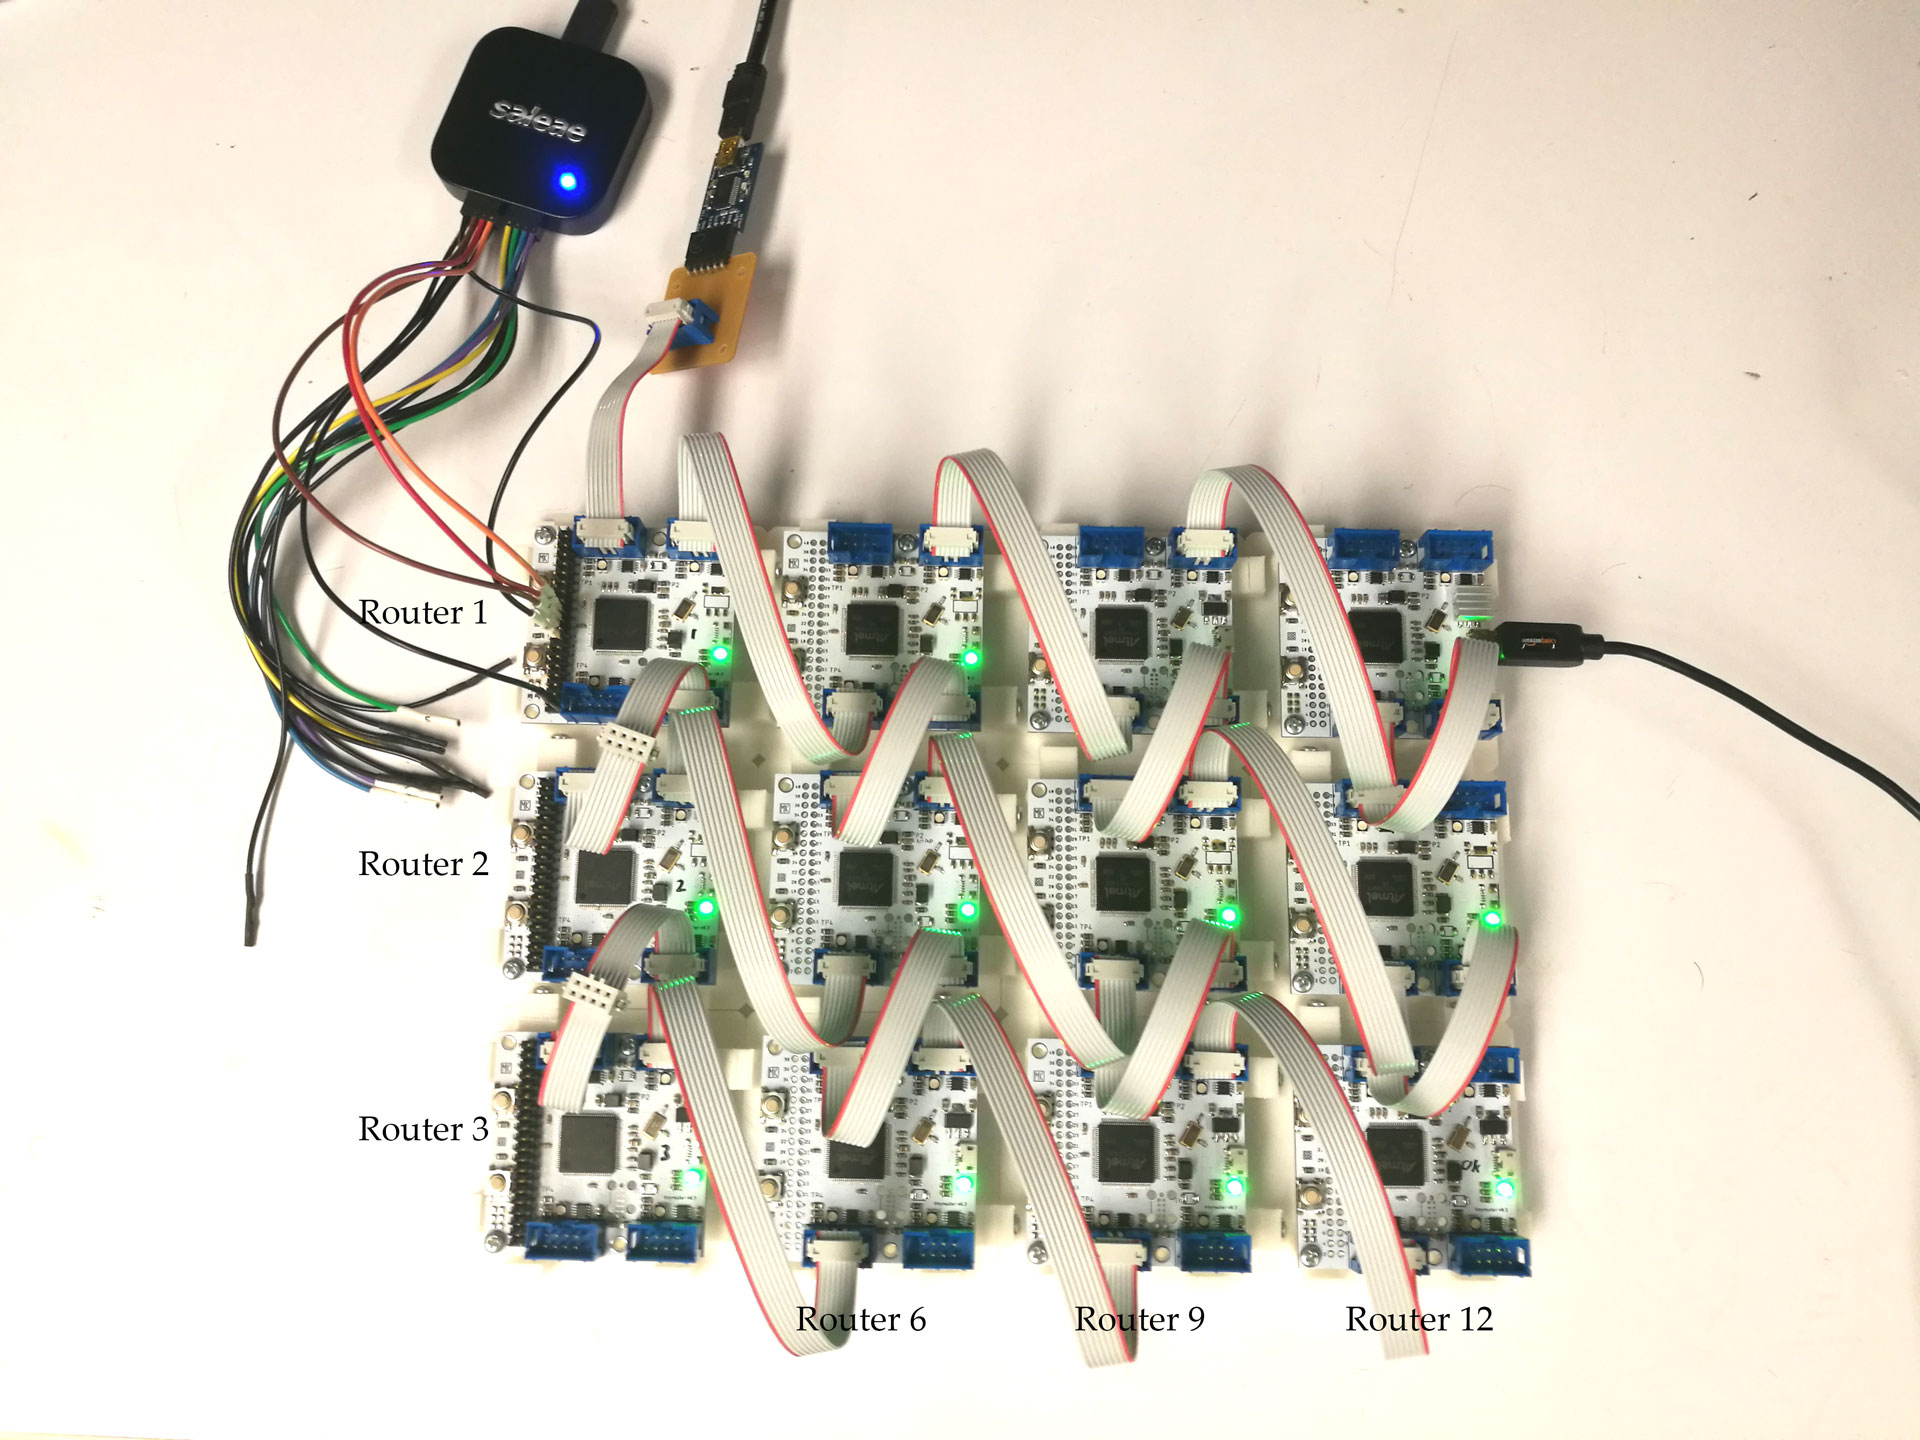
\includegraphics[width=\linewidth]{figures/hardware-12_routers.jpg}
    \caption{The 12-router hardware testbed. Each router is an ATSAMS70-based TinyNet node. The Saleae Logic 8 logic analyzer (left) captures UART timing; the TinyNet Bridge (right, USB) provides host access. Routers are interconnected in a $3\times4$ grid topology.}
    \label{fig:12-routers}
\end{figure}
To assess multi-link routing performance, we assembled a network comprising 12 interconnected TinyNet routers. This setup is illustrated in Fig.~\ref{fig:12-routers}, along with the logic analyzer used for timing Round-Trip Time (RTT) and $\mathrm{D}_{\mathrm{packet}}$ and verifying $\mathrm{L}_{\mathrm{tt}}$. Additionally, a TinyNet Bridge is shown, enabling network access via USB Port. We measured the RTT between Router 1 and Router 12, finding an average RTT of $511\,\mu\mathrm{s}$, captured directly by the logic analyzer and shown in Fig.~\ref{fig:rtt-511us}. This hardware measurement is cross-validated by the simulation result of $505\,\mu\mathrm{s}$ (Section~\ref{sec:sim-val}), a discrepancy of only $1.2\%$, which provides strong corroborating evidence for the accuracy of both measurements.

\begin{figure}[th]
    \centering
    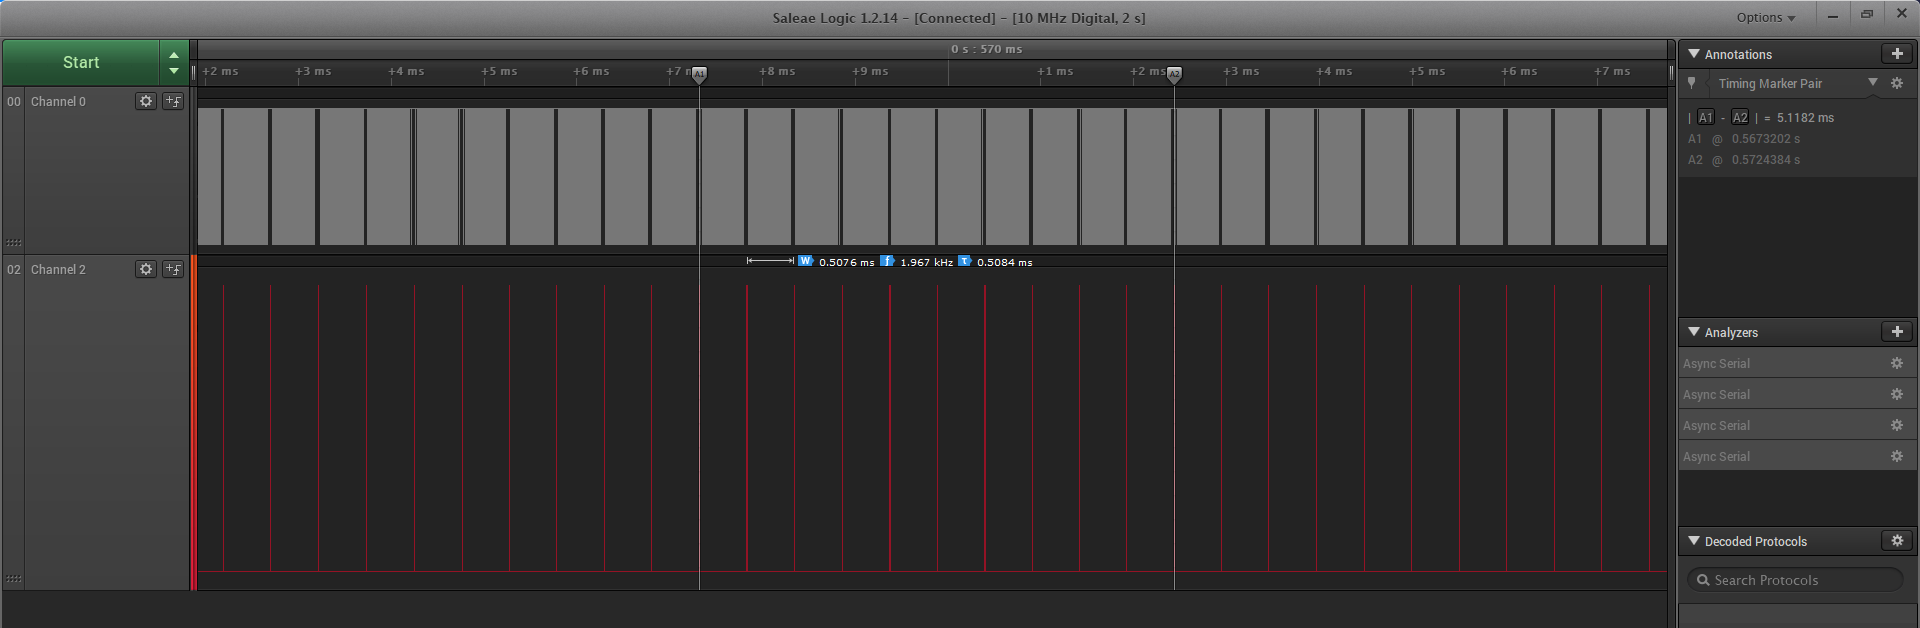
\includegraphics[width=\linewidth]{figures/results-rtt-511us.png}
    \caption{Logic-analyzer capture of the $511\,\mu\mathrm{s}$ round-trip time between Router~1 and Router~12 in the 12-router hardware testbed. The cursors mark the start of the outgoing packet and the end of the returning acknowledgement; this interval is the primary hardware calibration point for the simulation model.}
    \label{fig:rtt-511us}
\end{figure}

\subsection{Simulation Validation}
\label{sec:sim-val}
Our simulation, capable of representing various network topologies and traffic conditions, operates in JavaScript and leverages the open-source Simbit architecture \cite{simbit}. To validate the simulation's effectiveness, we emulate a 12-node grid network, mirroring our hardware setup. We initialize the simulated nodes with parameters derived from hardware measurements via the logic analyzer: processing delay $\mathrm{D}_{\mathrm{process}} = 37\,\mu\mathrm{s}$, per-byte interrupt time $\mathrm{D}_{\mathrm{byte}} = 1.5\,\mu\mathrm{s}$, and link bitrate $\mathrm{L}_{\mathrm{br}} = 20\,\mathrm{MHz}$. All simulations use $\lambda = 0.5$, a heartbeat transmission period of $1\,\mathrm{ms}$, and a missed-heartbeat detection window of $2\,\mathrm{ms}$. This process ensures that our simulation closely resembles real-world hardware operations.

We facilitate message transmission diagonally across the grid and record the round-trip time (RTT). Comparing the RTT of $511\,\mu\mathrm{s}$ obtained from our hardware tests with the simulation's RTT of $505\,\mu\mathrm{s}$, we observe a minor discrepancy of only $1.2\%$, confirming that the simulation accurately reproduces hardware behavior at this operating point. RTT variance and failure-recovery statistics reported in subsequent sections are derived from simulation; hardware validation of these statistics remains future work.

\subsection{Simulation Sensitivity Analysis}
\label{sec:sensitivity}

To bound the effect of hardware timing uncertainty on the reported variance results, we conducted a one-at-a-time sensitivity analysis, independently perturbing each of the three calibrated parameters---$\mathrm{D}_{\mathrm{process}}$, $\mathrm{D}_{\mathrm{byte}}$, and $\mathrm{L}_{\mathrm{br}}$---by $\pm30\%$ from their hardware-measured values and re-running the 10-kHz cross-traffic scenario on the 4$\times$4 grid.

\begin{table}[h]
	\centering
	\caption{Sensitivity of per-hop RTT mean and standard deviation to $\pm30\%$ perturbation of hardware timing parameters. Baseline: $\mathrm{D}_{\mathrm{process}} = 37\,\mu\mathrm{s}$, $\mathrm{D}_{\mathrm{byte}} = 1.25\,\mu\mathrm{s}$, $\mathrm{L}_{\mathrm{br}} = 20\,\mathrm{MHz}$.}
	\label{tab:sensitivity}
	\begin{tabular}{||l|r|r||}
		\hline
		Configuration & Mean ($\mu$s) & $\sigma$ ($\mu$s) \\\hline\hline
		Baseline & 188 & 87 \\
		$\mathrm{D}_{\mathrm{process}} -30\%$ & 53 & 20 \\
		$\mathrm{D}_{\mathrm{process}} +30\%$ & 887 & 392 \\
		$\mathrm{D}_{\mathrm{byte}} -30\%$ & 138 & 56 \\
		$\mathrm{D}_{\mathrm{byte}} +30\%$ & 253 & 98 \\
		$\mathrm{L}_{\mathrm{br}} -30\%$ & 228 & 90 \\
		$\mathrm{L}_{\mathrm{br}} +30\%$ & 217 & 96 \\
		\hline
	\end{tabular}
\end{table}

Bitrate uncertainty has the least influence: a $\pm30\%$ change in $\mathrm{L}_{\mathrm{br}}$ produces at most an 11\% change in $\sigma$. Per-byte interrupt time has moderate influence ($\sigma$ changes $-36\%$ to $+13\%$). Processing delay has the strongest influence: a $+30\%$ perturbation drives the network toward saturation at this traffic level, indicating operation near the processing-capacity boundary.

$\mathrm{D}_{\mathrm{process}}$ is validated by two independent methods: direct logic-analyzer measurement ($37\,\mu\mathrm{s}$) and analytical derivation from the MCU's interrupt service routine (450~cycles $\div$ 300~MHz per-byte, with the forwarding path executing a deterministic instruction sequence). The 1.2\% RTT match at the hardware calibration point confirms this value, bounding the practical uncertainty in $\mathrm{D}_{\mathrm{process}}$ to well under 30\%. The parameters for which the analysis shows benign sensitivity---$\mathrm{D}_{\mathrm{byte}}$ and $\mathrm{L}_{\mathrm{br}}$---are less tightly constrained by independent measurement but do not materially affect the reported results within their plausible uncertainty ranges.

\subsection{Determinism of Communication Time}
A crucial measure of TinyNet's effectiveness is communication time determinism, specifically the standard deviation of the round trip time for each hop a message makes. Different from previous systems that relied on spanning tree models, TinyNet thrives in more extensive network topologies. Therefore, our evaluation focuses on both determinism and robustness within a compact grid setting.

\subsubsection{Evaluation in a 4-by-4 Grid}
\begin{figure}[th]
    \centering
    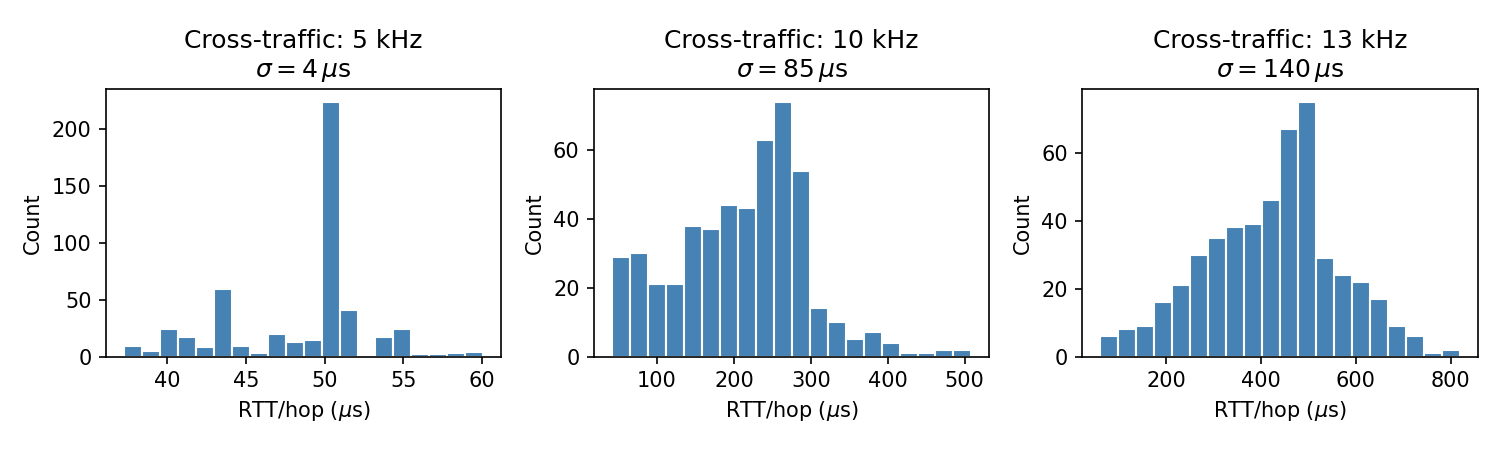
\includegraphics[width=\linewidth]{figures/pdf_grid_cross.png}
    \caption{Per-packet RTT histograms ($x$-axis in $\mu$s) in a 4$\times$4 grid, simulated over 30~ms. Main flow: 5~kHz from node~0 to node~15. Cross-traffic on the opposite diagonal (node~3 to node~12) at 5~kHz (top), 10~kHz (middle), and 13~kHz (bottom). Standard deviations: $\sigma = 4$, 85, and $140\,\mu\mathrm{s}$, respectively.}
    \label{fig:hists-cross}
\end{figure}
We begin by simulating a 4-by-4 grid of nodes, with each node having a packet delay time of $37 \mu \mathrm{s}$ (the hardware-measured $\mathrm{D}_{\mathrm{process}}$) and each link operating at a bitrate of 20 MHz. We transmit crucial messages diagonally across the grid at 5 kHz for 30 ms. Simultaneously, we model varying levels of cross-traffic on the opposite diagonal: 5 kHz, 10 kHz, and 13 kHz in separate simulations. The resulting histograms of per-packet round trip times are shown in Fig.~\ref{fig:hists-cross}, with standard deviations of $4 \mu \mathrm{s}$, $85 \mu \mathrm{s}$, and $140 \mu \mathrm{s}$ for each traffic scenario, respectively.

\subsubsection{Evaluation in a Simulated Airplane Wing Network}
\begin{figure}[th]
    \centering
    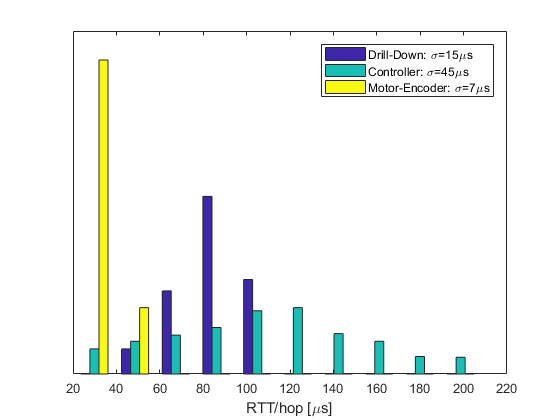
\includegraphics[width=\linewidth]{figures/pdf_RTT.png}
    \caption{Per-hop RTT histograms ($x$-axis in $\mu$s) in a simulated airplane wing topology: one master node, three controllers, 24 motors, and 24 encoders, simulated over 30~ms. Standard deviations: master--encoder queries $\sigma = 15\,\mu\mathrm{s}$, controller--motor loops $\sigma = 45\,\mu\mathrm{s}$, motor--encoder loops $\sigma = 7\,\mu\mathrm{s}$.}
    \label{fig:hists-airplane}
\end{figure}
In addition, we assess determinism within a simulated airplane wing network, structured into four layers: a single master node on top, three controllers in the second layer, each connected to eight motors in the third layer, and each motor linked to two neighboring motors and an encoder in the fourth layer. Under the same hardware parameters as the grid, the motors maintain a 2.5-kHz control loop with their encoders, the controllers manage a 1-kHz loop with each motor, and the master node queries each encoder at 500 Hz. This simulation, conducted over 30 ms, reveals per-hop round trip times as illustrated in Fig.~\ref{fig:hists-airplane}, with a standard deviation of $15 \mu \mathrm{s}$ for master-encoder queries, $45 \mu \mathrm{s}$ for controller-motor loops, and $7 \mu \mathrm{s}$ for motor-encoder loops.

These results highlight two key outcomes:
\begin{itemize}
    \item \textbf{Impact of Network Traffic on Determinism:} An increase in network traffic tends to reduce network determinism. As the number of packets traversing the network grows, so does the buffer depth at individual nodes, leading to increased message latency and variability in latency. This relationship is compounded by path length: networks with more routing hops expose each packet to more opportunities for queuing, so determinism degrades faster per unit of added traffic in larger networks. This is consistent with the airplane wing results, where the short motor-encoder paths (few hops) achieve $\sigma = 7\,\mu\mathrm{s}$ while the longer master-encoder paths (many hops) exhibit $\sigma = 15\,\mu\mathrm{s}$ under similar per-link traffic loads.
    \item \textbf{TinyNet's Adaptability:} Despite the challenges of heavy cross-traffic, TinyNet maintains a high level of message determinism. Its dynamic adaptation to changing traffic conditions across different network areas effectively distributes the load among numerous nodes. This approach not only reduces message delivery time but also helps in consistently maintaining low latency levels.
\end{itemize}

\subsection{Robustness to Node Failure}
\label{sec:robustness}
\begin{figure}[th]
    \centering
    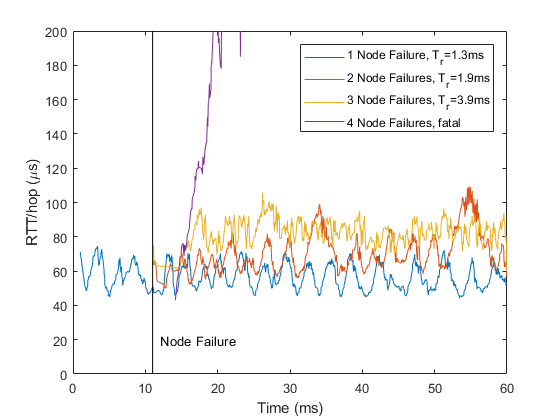
\includegraphics[width=\linewidth]{figures/node_failure_recovery.png}
    \caption{Per-packet RTT ($y$-axis in $\mu$s, $x$-axis in ms over 0--30~ms window) in the 4$\times$4 grid before and after random interior node removal at $t=11\,\mathrm{ms}$. Colors denote failure count: 1~node (blue), 2~nodes (orange), 3~nodes (green), 4~nodes (red). Recovery times (RTT returning to within $2\times$ pre-failure mean): 1.3~ms, 1.9~ms, and 3.9~ms for 1, 2, and 3 node failures, respectively. Four-node removal (25\%) did not converge within the simulation window.}
    \label{fig:failure}
\end{figure}
Robustness to node failure is the second crucial dimension of TinyNet's performance, focusing on the network's ability to rapidly respond to and recover from node failures. For assessing this essential aspect, we conducted simulations on a 4-by-4 grid of nodes, using the same hardware parameters as in our message determinism evaluation. In these simulations, corner nodes sent messages diagonally across the grid at frequencies of 10 kHz and 5 kHz. At 11 milliseconds into the simulation, we randomly disconnected one, two, three, or four nodes simultaneously (chosen uniformly at random from the interior nodes of the grid), then observed and recorded the subsequent message delay times. Each failure-count condition was repeated across multiple independent trials with different randomly selected node sets, and the reported recovery times represent the average across those trials. Recovery is defined as the point at which the per-packet delay returns to within $2\times$ of its pre-failure mean. The findings, depicted in Fig.~\ref{fig:failure}, show per-packet delay over time with the failure event at $t = 11\,\mathrm{ms}$. After a single node failure, the network recovered in 1.3 ms; after two failures, in 1.9 ms; and after three failures, in 3.9 ms.

Key observations from these results include:
\begin{itemize}
    \item \textbf{Rapid Recovery from Failures:} TinyNet recovers from node failures within 1.3--3.9~ms. Even with approximately 19\% of the network (3 of 16 nodes) failing simultaneously, TinyNet maintains round trip times effectively. By contrast, the stateful LFA baseline drops approximately 250 packets during the 50~ms BFD cutover window before routing resumes (see Section~\ref{sec:comparison}).
    \item \textbf{Impact of Multiple Node Failures:} The loss of a single node does not significantly affect long-term communication. However, multiple node failures can adversely affect both message latency and network determinism. This outcome is predictable as TinyNet's load-balancing capabilities are most effective when there are sufficient alternative nodes for message rerouting.
    \item \textbf{Capacity for Message Maintenance in Failures:} TinyNet sustains message transmission even under substantial network failures. In contrast to spanning-tree protocols, which lose connectivity to entire sub-trees on a single node failure~\cite{spb}, TinyNet reroutes around failed nodes by flooding. However, recovery did not converge within the simulation window at a 25\% failure rate (4 of 16 nodes simultaneously), indicating that sufficient path redundancy is a prerequisite for TinyNet's rerouting to succeed.
\end{itemize}

\subsection{Comparison Against a Stateful Routing Baseline}
\label{sec:comparison}
\begin{figure}[th]
    \centering
    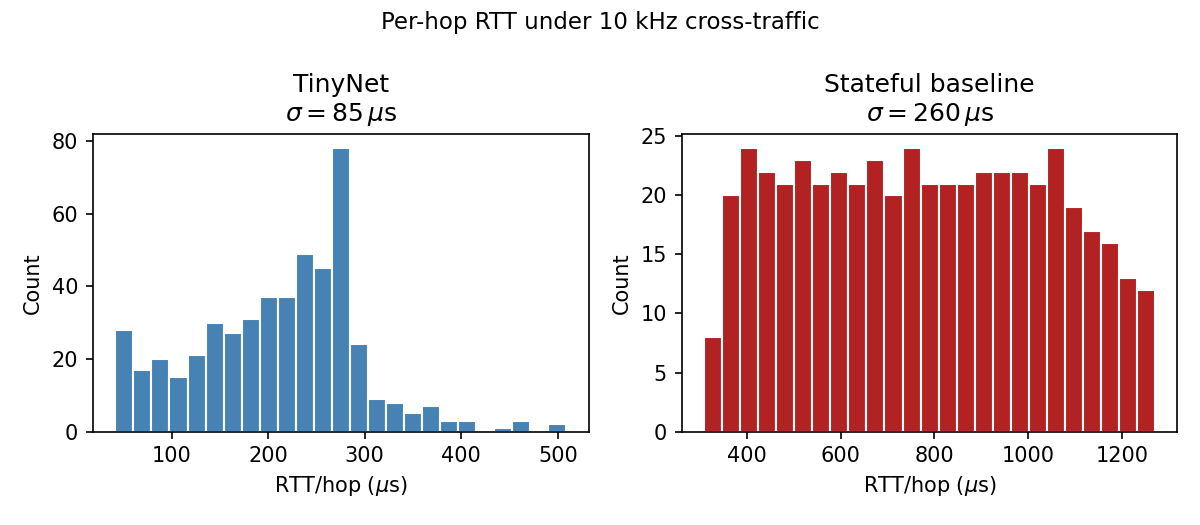
\includegraphics[width=\linewidth]{figures/comparison_cross.png}
    \caption{Per-hop RTT histograms ($x$-axis in $\mu$s) under 10~kHz cross-traffic on the 4$\times$4 grid: TinyNet (left, $\sigma = 85\,\mu\mathrm{s}$) versus stateful shortest-path baseline (right, $\sigma = 139\,\mu\mathrm{s}$), a 39\% reduction in variability.}
    \label{fig:comparison-cross}
\end{figure}
\begin{figure}[th]
    \centering
    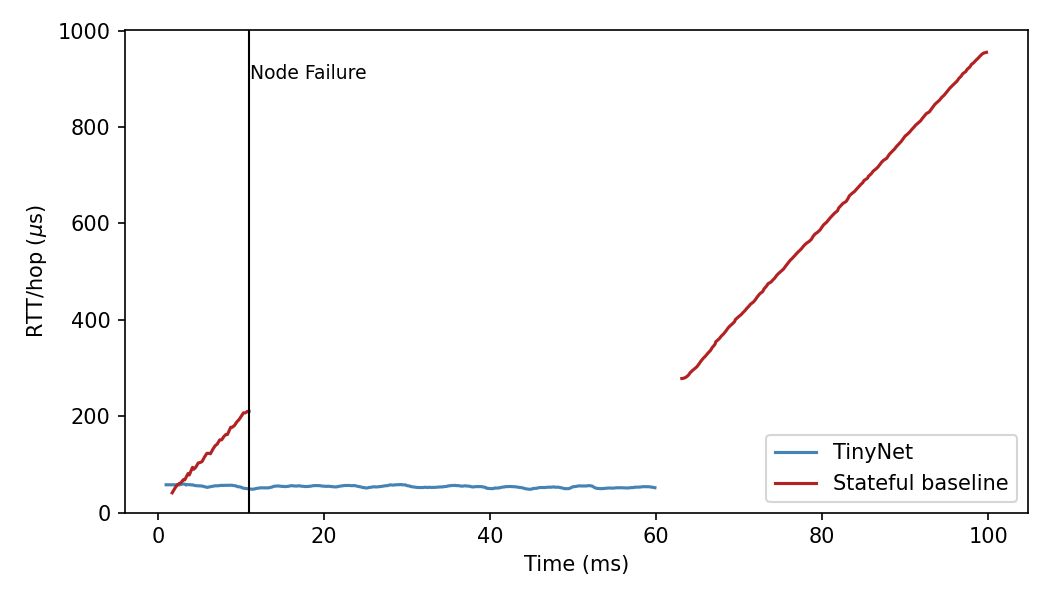
\includegraphics[width=\linewidth]{figures/comparison_failure.png}
    \caption{Cumulative packets delivered ($y$-axis, 0--30~ms window on $x$-axis) following a single interior node failure at $t=11\,\mathrm{ms}$: TinyNet (blue) versus LFA-style stateful baseline (red). Both lines overlap before the failure. TinyNet misses fewer than 20 packets and recovers in $\approx\!3\,\mathrm{ms}$; the baseline's 50~ms flat segment (packets dropped during BFD detection and LFA cutover) represents $\approx\!250$ undelivered packets.}
    \label{fig:comparison-failure}
\end{figure}

To directly address the question of how TinyNet compares against stateful routing, we implemented a shortest-path baseline in our JavaScript simulator. The baseline pre-computes BFS shortest paths at startup and routes each packet along the single lowest-hop-count path, with no multipath. On link failure, it drops all packets destined for affected nodes for 50\,ms---the typical BFD detection plus LFA switchover window \cite{rfc5286,cisco_lfa}, and the current best-case for stateful IP Fast Reroute (see Section~\ref{sec:related:frr})---before recomputing routes. We compare against LFA rather than RPL because LFA represents the fastest-recovering class of stateful protocols in production use; RPL's DODAG repair mechanism targets energy-constrained wireless links and operates on a fundamentally different latency regime not directly applicable to UART-connected NCS (see Section~\ref{sec:related:mesh}).

\subsubsection{RTT Determinism Under Cross-Traffic}
Fig.~\ref{fig:comparison-cross} shows per-hop RTT histograms under 10 kHz cross-traffic for both protocols on the same 4-by-4 grid. TinyNet achieves a standard deviation of $85\,\mu\mathrm{s}$, compared to $139\,\mu\mathrm{s}$ for the stateful baseline---a $39\%$ reduction in variability. The improvement stems from TinyNet's cost function actively redistributing packets across multiple paths in response to buffer occupancy, whereas the stateful baseline funnels all traffic through a single fixed path, allowing congestion to build without relief.

\subsubsection{Failure Recovery}
Fig.~\ref{fig:comparison-failure} shows cumulative packets delivered following a single node failure at $t=11\,\mathrm{ms}$. Before the failure both protocols deliver at the same rate; the lines overlap. After the failure, TinyNet recovers in approximately 3\,ms as packets immediately flood to alternate paths, missing fewer than 20 packets in total. (The 1.3\,ms single-failure figure reported in Section~\ref{sec:robustness} is measured by a different metric---per-packet RTT returning to within $2\times$ of its pre-failure mean---under dual diagonal traffic at 10\,kHz plus 5\,kHz; the 3\,ms figure here is read from the cumulative delivery curve under 5\,kHz single-diagonal traffic and therefore reflects a different saturation point.) The stateful baseline's cumulative count is flat for 50\,ms---the LFA detection and cutover window \cite{rfc5286,cisco_lfa}---before routing resumes; this 50\,ms flat segment is the expected, designed behavior of LFA: during BFD timeout, packets destined for the failed path are dropped, and the baseline does not resume delivery until the cutover completes. This flat segment represents approximately 250 undelivered packets. This more-than-order-of-magnitude difference in recovery time (3\,ms vs.\ 50\,ms) reflects the fundamental asymmetry between TinyNet's data-driven reroute and LFA's pre-computed backup activation: TinyNet's first post-failure packet triggers flooding immediately, while LFA must wait for BFD to time out before switching to its pre-installed alternate.